\section{LAPIS: Location-Aware Privacy--Information Selection}
\label{sec:lapis}
Algorithm~\ref{alg:lapis} evaluates a finite grid and selects one fixed reporting budget. The grid, scenarios, prior, beam map, sample counts, and confidence levels are fixed before evaluation; no monotonic outage or convex objective is assumed.

\begin{algorithm}[t]
\caption{LAPIS: Fixed Privacy-Budget Selection}
\label{alg:lapis}
\footnotesize
\begin{algorithmic}[1]
\REQUIRE Public scenarios, prior/weights, grid $\mathcal E$, mode and constraint; $N_s,N_c,\delta_s,\delta_c$.
\ENSURE Fixed $\epsilon^\star$, confirmation interval/status, and (P1) gap $G$; or no candidate.
\STATE Set $\mathcal C=\mathcal E$; for (P1), retain $\epsilon r_0\le\eta_{\max}$.
\STATE If $\mathcal C=\varnothing$, \textbf{return} grid-infeasible.
\STATE Draw i.i.d. report-noise seeds and true-channel samples; reuse across budgets.
\FOR{each $\epsilon\in\mathcal C$}
 \STATE Generate reports; apply MAP and the frozen beam map.
 \STATE Evaluate true-channel outages via~\eqref{eq:success}; estimate $\widehat q_{\epsilon j}$ for each scenario by~\eqref{eq:paired-outage}.
 \STATE Compute $[L_\epsilon,U_\epsilon]$ via~\eqref{eq:outage-confidence}--\eqref{eq:aoii-confidence}.
\ENDFOR
\IF{mode is (P1)}
 \STATE Select $\epsilon^\star$ and compute $G$ by~\eqref{eq:lapis-p1}; ties favor smaller budgets.
\ELSE
 \STATE Set $\mathcal F_D=\{\epsilon\in\mathcal C:U_\epsilon\le D_{\max}\}$.
 \STATE If $\mathcal F_D=\varnothing$, \textbf{return} infeasible when $\min L_\epsilon>D_{\max}$, otherwise unconfirmed; else set $\epsilon^\star=\min\mathcal F_D$.
\ENDIF
\STATE Freeze $\epsilon^\star$; evaluate with $N_c$ new samples per scenario and radius $d_c$ to obtain $[L_c,U_c]$.
\STATE \textbf{return} budget, interval, (P1) privacy status and $G$, or (P2) confirmation iff $U_c\le D_{\max}$; retain the selected budget.
\end{algorithmic}
\end{algorithm}

\subsection{Paired Outage Evaluation}
For each scenario $j$ and sample $\ell$, draw $R_{j\ell}\sim\mathrm{Gamma}(3,1)$, a uniform unit-sphere direction $\mathbf U_{j\ell}$, and independent true-channel samples from~\eqref{eq:channel} or the frozen empirical CSI bank. Reuse these draws across budgets, setting
\begin{align}
 \mathbf z_{j\ell}(\epsilon)
 &=\mathbf x_j+\frac{R_{j\ell}}{\epsilon}\mathbf U_{j\ell},\nonumber\\
 \widehat q_{\epsilon j}
 &=\frac1{N_s}\sum_{\ell=1}^{N_s}(1-Y_{j\ell}(\epsilon)).
 \label{eq:paired-outage}
\end{align}
Each $Y_{j\ell}(\epsilon)$ is computed through~\eqref{eq:map}--\eqref{eq:success} on the same true channel realization. This coupling preserves the marginal distributions and independence across $\ell$. Let $F_\alpha(q)$ denote the right-hand side of~\eqref{eq:mean-aoii}. The plug-in estimate is $\widehat J(\epsilon)=\sum_j\omega_jF_\alpha(\widehat q_{\epsilon j})$.

To account for finite-sample uncertainty, Hoeffding's inequality~\cite{hoeffding1963} and a union bound over $N_{\mathrm x}|\mathcal E|$ pairs give the simultaneous radius
\begin{equation}
 \begin{gathered}
 d_s=\sqrt{\frac{\log(2N_{\mathrm x}|\mathcal E|/\delta_s)}{2N_s}},\\
 q^-_{\epsilon j}=[\widehat q_{\epsilon j}-d_s]_+,\quad
 q^+_{\epsilon j}=\min\{1,\widehat q_{\epsilon j}+d_s\},
 \end{gathered}
 \label{eq:outage-confidence}
\end{equation}
where $[a]_+=\max\{0,a\}$ and $\delta_s\in(0,1)$. Since $F_\alpha$ is increasing, with probability at least $1-\delta_s$, every candidate satisfies
\begin{equation}
 \begin{gathered}
 L_\epsilon=\sum_j\omega_jF_\alpha(q^-_{\epsilon j}),\quad
 U_\epsilon=\sum_j\omega_jF_\alpha(q^+_{\epsilon j}),\\
 L_\epsilon\le J(\epsilon)\le U_\epsilon.
 \end{gathered}
 \label{eq:aoii-confidence}
\end{equation}
These bounds quantify Monte Carlo error conditional on the prescribed map and channel model. Model mismatch requires a separate assessment.

\subsection{Selection and Independent Confirmation}
For (P1), form $\mathcal F_\eta=\{\epsilon\in\mathcal E:\epsilon r_0\le\eta_{\max}\}$ and choose
\begin{equation}
 \begin{gathered}
 \epsilon^\star\in\arg\min_{\epsilon\in\mathcal F_\eta}U_\epsilon,\\
 G=U_{\epsilon^\star}-\min_{\epsilon\in\mathcal F_\eta}L_\epsilon.
 \end{gathered}
 \label{eq:lapis-p1}
\end{equation}
On the simultaneous-coverage event, $J(\epsilon^\star)-\min_{\epsilon\in\mathcal F_\eta}J(\epsilon)\le G$; $G$ bounds unresolved grid suboptimality.

For (P2), choose the smallest $\epsilon$ satisfying $U_\epsilon\le D_{\max}$. If none qualifies, $\min_\epsilon L_\epsilon>D_{\max}$ indicates grid infeasibility on the coverage event; otherwise feasibility is unconfirmed. An interval straddling the threshold leaves grid optimality unresolved.

Freeze the budget and use $N_c$ independent samples per scenario, replacing $d_s$ in~\eqref{eq:outage-confidence}--\eqref{eq:aoii-confidence} by $d_c=\sqrt{\log(2N_{\mathrm x}/\delta_c)/(2N_c)}$. For (P2), confirm feasibility only if the new upper endpoint is at most $D_{\max}$; otherwise report unconfirmed and retain the selected budget. The union-bound coverage for selection and confirmation is at least $1-\delta_s-\delta_c$. For the geometry-based beam rule and brute-force MAP, selection costs $O(|\mathcal E|N_{\mathrm x}N_s(N_{\mathrm x}+M))$, followed by one-candidate confirmation. Figures~\ref{fig:arrays} and~\ref{fig:selection} examine array sensitivity and selection reliability. 

\begin{figure*}[!t]
\centering
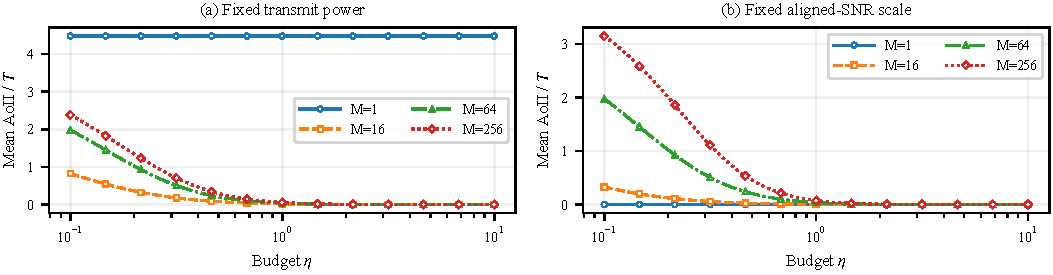
\includegraphics[width=\textwidth]{Figs/array_effect.pdf}
\caption{Geometric Rician array controls. Fixed power uses reference single-element SNR $-5$~dB at 150~m. The second control fixes reference LOS aligned-SNR scale at 13.06~dB, adjusting power as $1/M$.}
\label{fig:arrays}
\end{figure*}
\begin{figure*}[!t]
\centering
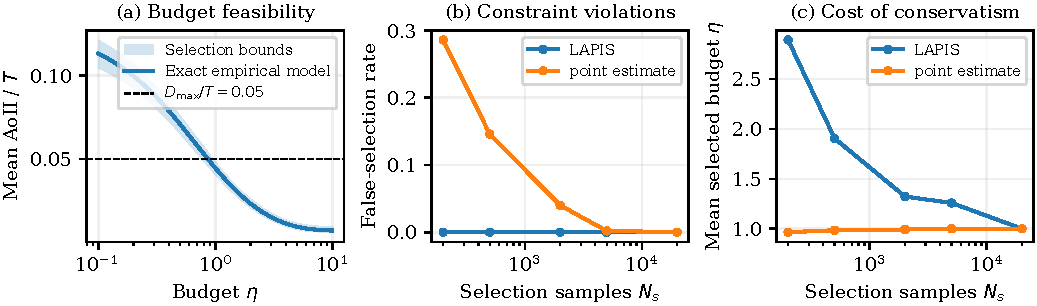
\includegraphics[width=\textwidth]{Figs/selection_reliability.pdf}
\caption{Conditional empirical-model selection. Reliability uses equivalent Bernoulli links, independent budget streams, and 1,000 repetitions at each of 13 sample sizes. Both methods use identical selection samples and grids. Panel (b) reports selections that violate the exact-model constraint; panel (c) shows their disclosure cost.}
\label{fig:selection}
\end{figure*}
